\documentclass{article}

\usepackage{fullpage}  % Makes the text margins smaller
\usepackage{graphicx} % To include figures
\usepackage{fancyvrb} % Includes the \VerbatimInput command to read in code files
\usepackage{rotating}  % To make sideways figures
\usepackage{hyperref}

\author{Cody Lieu, Yixin Lin}
\title{COMPSCI 527 Homework 3}

\begin{document}
\maketitle

\section*{Problem 1(a)}

\VerbatimInput[fontsize=\small,fontshape=n,xleftmargin=15mm]{compress.m}

We made a figure, but we plot over it repeatedly in the following questions. If you want to see what it looks like, look at those.

\section*{Problem 1(b)}

$$\sigma^2  = [4.2282 0.2427 0.0782 0.0238]^T $$

Since we project down to the first two dimensions, the fraction of the variance is $$\frac{4.2282 + 0.2427}{4.2282 + 0.2427 + 0.0782 + 0.0238} = 0.97769468$$. So the percentage of variance we capture with our PCA to 2 dimensions is $97.7769\%$.

\section*{Problem 2(a)}

\VerbatimInput[fontsize=\small,fontshape=n,xleftmargin=15mm]{trainTree.m}

\section*{Problem 2(b)}

\VerbatimInput[fontsize=\small,fontshape=n,xleftmargin=15mm]{treePartition.m}

\begin{center}
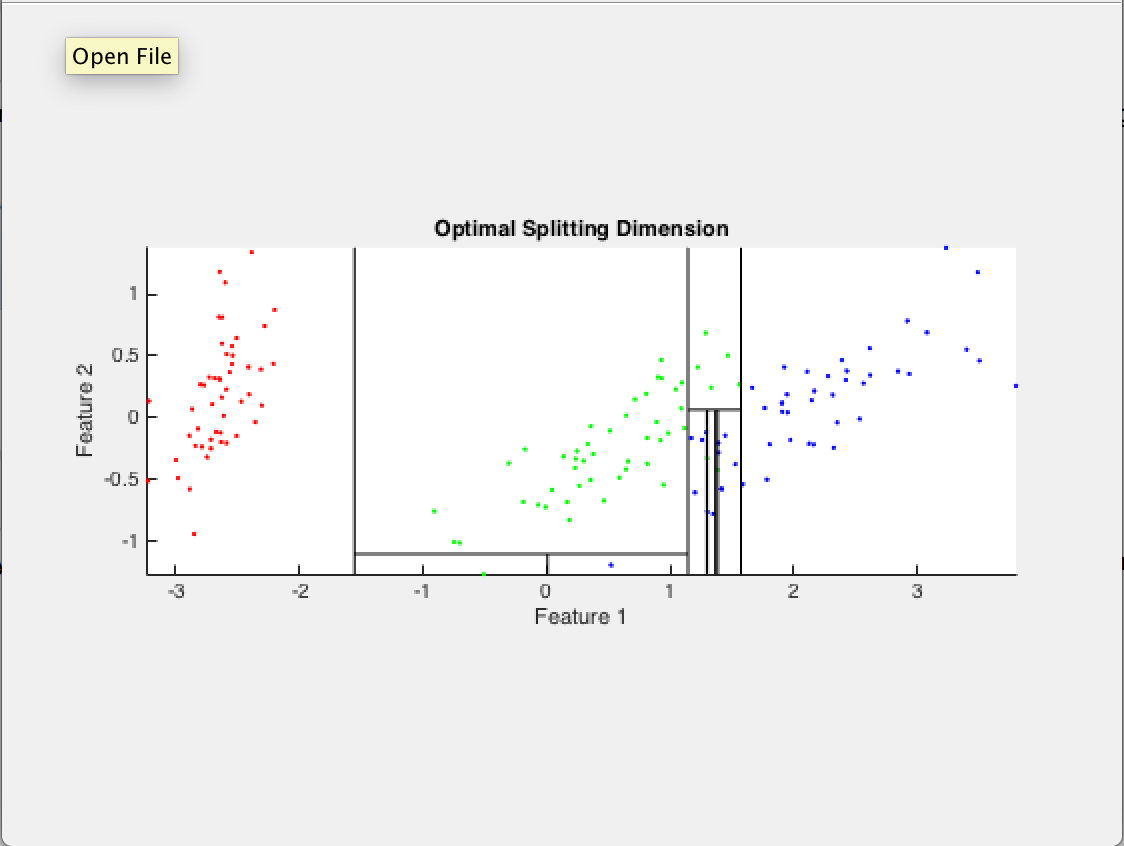
\includegraphics[width=0.8\textwidth]{2b_optimal_splitting_dimension.png}
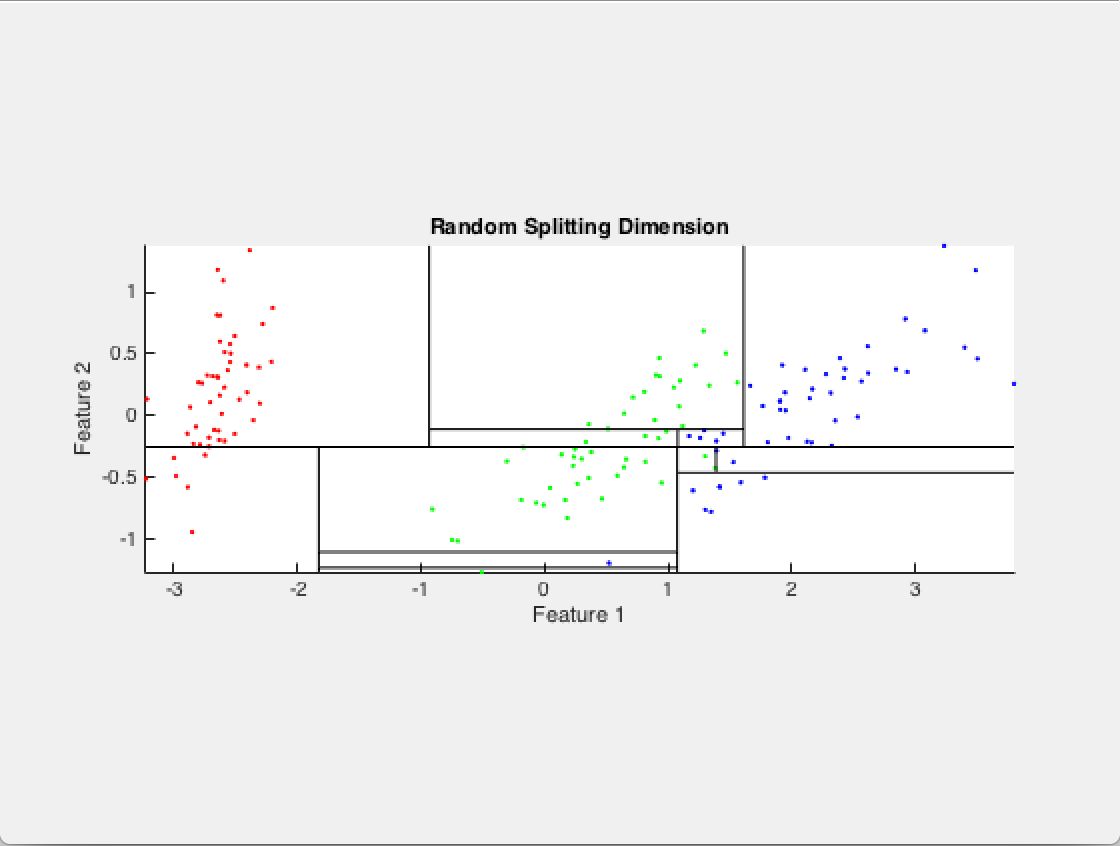
\includegraphics[width=0.8\textwidth]{2b_random_splitting_dimension.png}
\end{center}

\section*{Problem 3(a)}

\VerbatimInput[fontsize=\small,fontshape=n,xleftmargin=15mm]{treeClassify.m}

\section*{Problem 3(b)}

\VerbatimInput[fontsize=\small,fontshape=n,xleftmargin=15mm]{err.m}

All training errors are 0.

\section*{Problem 3(c)}

The training errors are 0, which makes sense since we didn't limit the depth of the tree or the minimum number of training samples in a leaf, which means we will keep adding nodes until we have 0 impurity (aka we classify all data in training set completely correctly).

\section*{Problem 3(d)}

\begin{center}
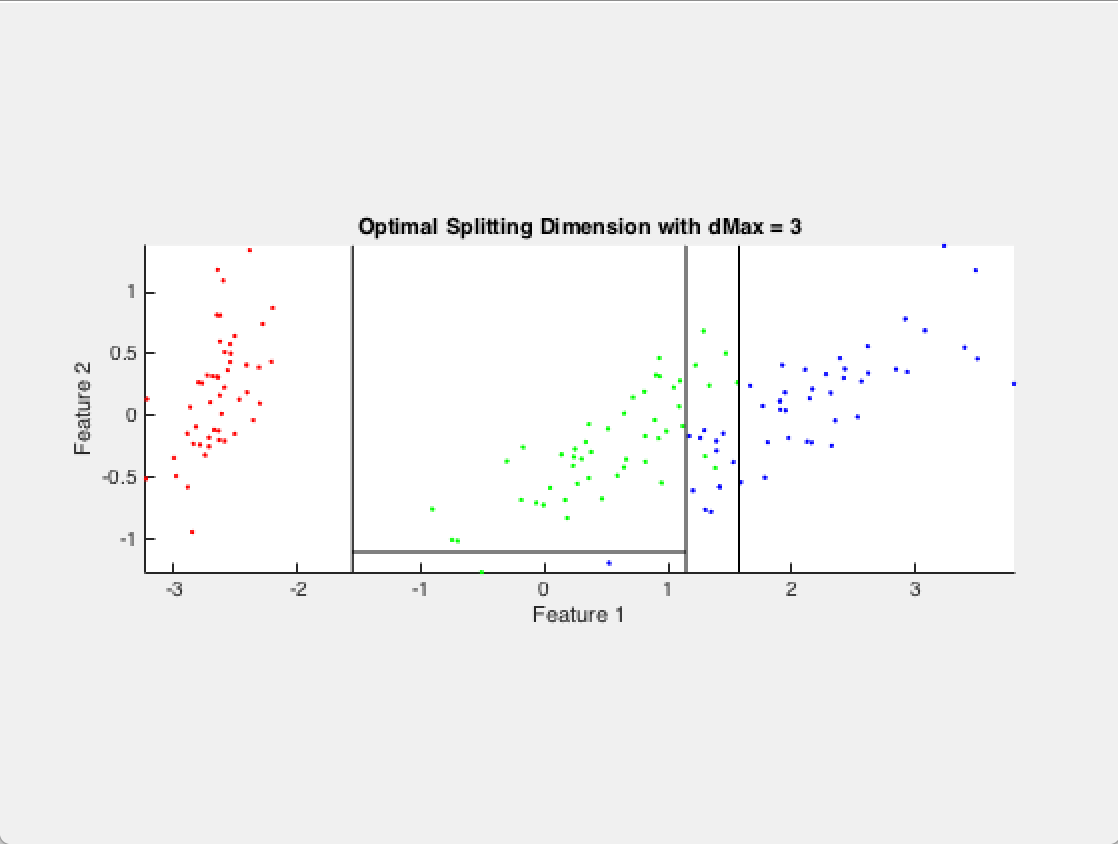
\includegraphics[width=0.8\textwidth]{3d_optimal_splitting_dimension.png}
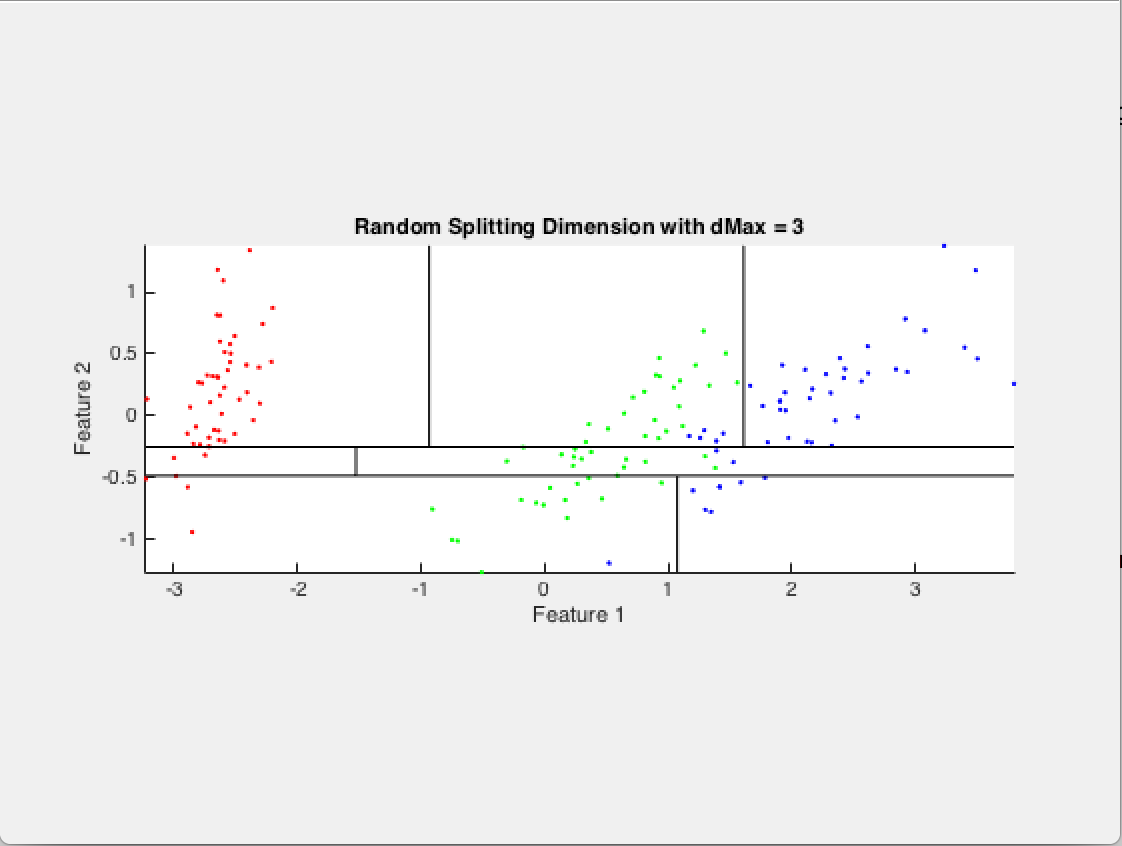
\includegraphics[width=0.8\textwidth]{3d_random_splitting_dimension.png}
\end{center}

The error rates are positive, which makes sense since we are limiting the depth of the tree. This means that the training of our model stops before we perfectly classify all the data in the training set.

Error rates with d-max = 3:

With optimal splitting dimension: 0.0533

With random splitting dimension: 0.0800

The first error rate is lower than the second, since we're picking the optimal splitting dimension each time instead of picking it at random.

\section*{Problem 3(e)}

\VerbatimInput[fontsize=\small,fontshape=n,xleftmargin=15mm]{cverr.m}

\section*{Problem 3(f)}

[0.0733    0.0800    0.1000    0.1000    0.0800]

The values aren't the same because k-fold cross validation uses k random samples of the data as buckets. This means that the resulting errors will be slightly different simply due to the random sampling process.

\section*{Problem 3(g)}

[0.0600    0.0600    0.0600    0.0600    0.0600]

The values are the same, which makes sense since leave-one-out cross validation always uses each datum as sample data once (i.e. each random partition is equivalent to another because each bucket only contains one datum).

\section*{Problem 3(h)}

The cross-validation method is called ``leave-one-out cross-validation''. This is the extreme version of k-fold classification, where the model is trained on each data point except N times. This gives us a lower variance on the estimated error. However, this is seldom used simply because we repeat the model-training N times, which is computationally very expensive.

\section*{Problem 3(i)}

\VerbatimInput[fontsize=\small,fontshape=n,xleftmargin=15mm]{3i.m}

Leave-one-out cross-validation errors: [0.2667 0.4867 0.0600 0.0467]

We would choose the first dimension, since the first dimension lets us get the smallest error rate.

\section*{Problem 3(j)}

The error rate for the previous classifier is worse than that of using the highest-variance feature from PCA, since using PCA would choose an equal or better axis that explains as much or more of the variance.

\section*{Problem 4(a)}

\VerbatimInput[fontsize=\small,fontshape=n,xleftmargin=15mm]{ctreePartition.m}

\begin{center}
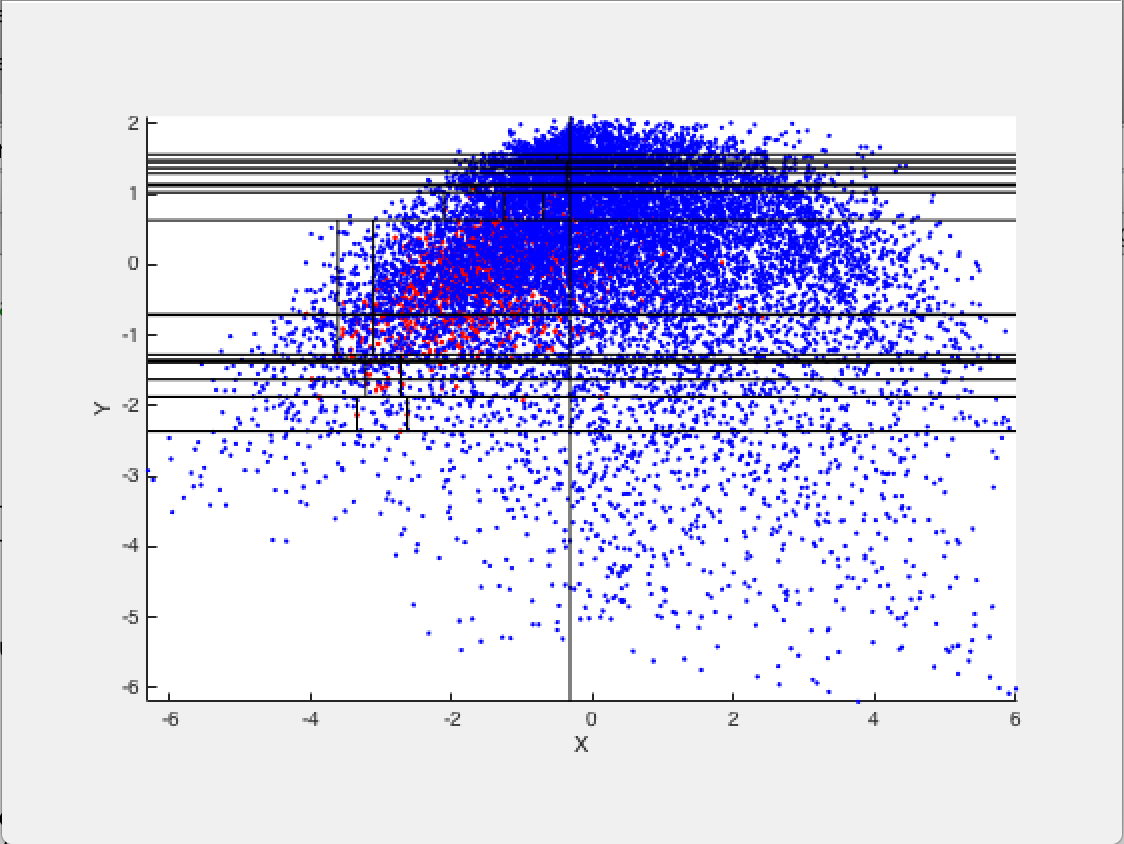
\includegraphics[width=0.8\textwidth]{4a.png}
\end{center}

\section*{Problem 4(b)}

We don't expect low generalization error rate, since a single tree is a weak classifier. This is because it's only trained on a random subset of the data. This is also empirically supported by our plot, which shows that the single forest misclassifies a large number of the total dataset.

\section*{Problem 4(c)}

\begin{center}
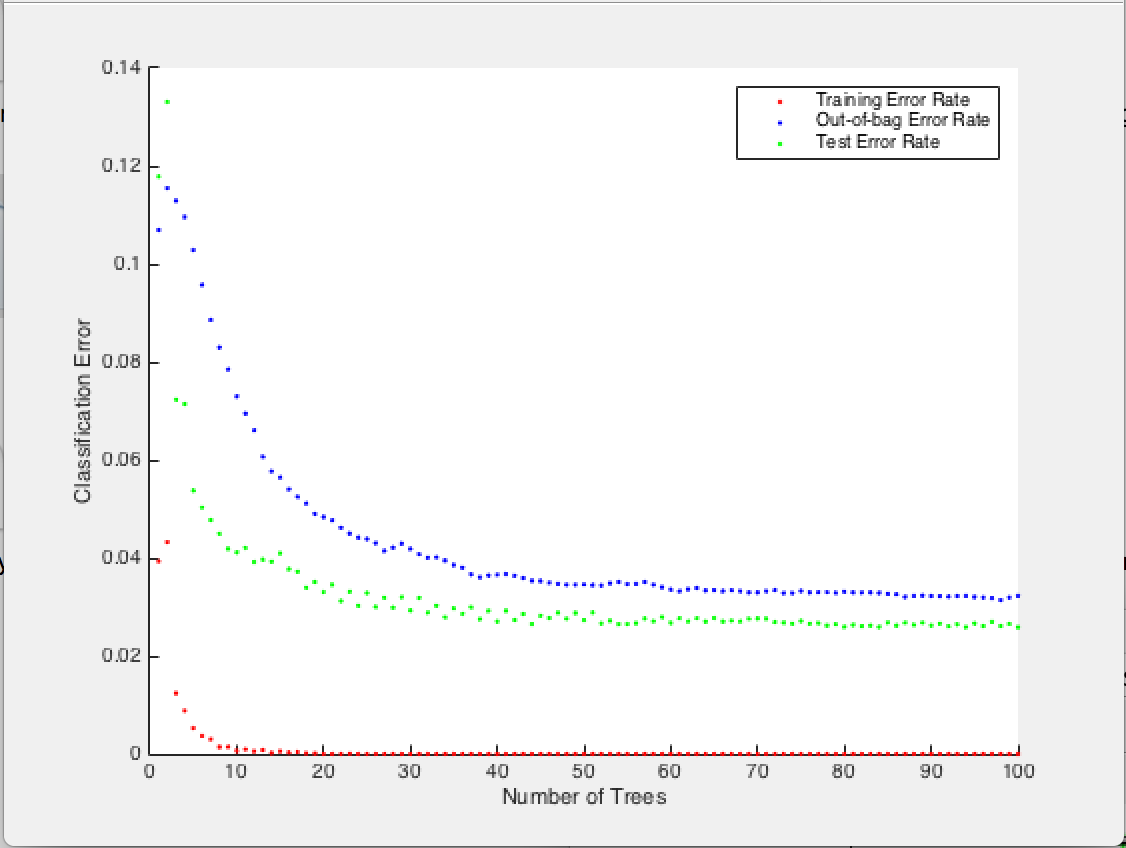
\includegraphics[width=0.8\textwidth]{4c.png}
\end{center}

\section*{Problem 4(d)}

Out-of-bag error rate and test error rate are good estimates of the generalization error, since they measure the error rate of the model on data it hasn't trained on. (Training error drops to zero quite fast, which isn't connected to generalization rate since training error depends on how well the model does on data it's trained on.) The shape of these plots tell us that random forests tend not to overfit (i.e. they generalize quite well), since the generalization error rate doesn't increase as the model complexity increases.

\section*{Problem 4(e)}

\begin{center}
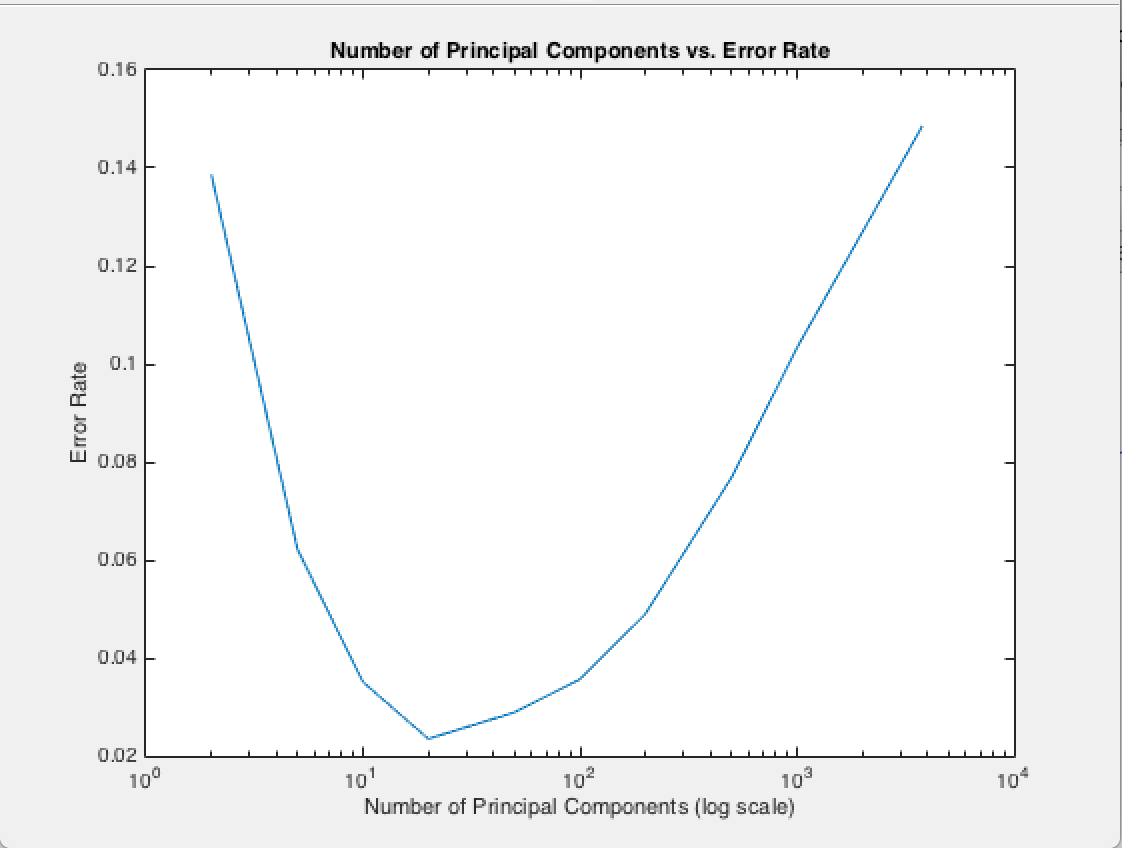
\includegraphics[width=0.8\textwidth]{4e.png}
\end{center}

\section*{Problem 4(f)}

We would use 20 components, since that's the number that gives us the least out-of-bag error rate. PCA generally helps, since we throw away the dimensions that explain the least amount of variance.

However, PCA may also hurt by throwing away variance that helps the model (e.g. by losing spatial information in a certain dimension), for example when the last few dimensions (ranked by variance) are important for classification.

% explain why PCA hurts, see ``http://stats.stackexchange.com/questions/52773/what-can-cause-pca-to-worsen-results-of-a-classifier''

\section*{Problem 4(g)}

\VerbatimInput[fontsize=\small,fontshape=n,xleftmargin=15mm]{4g.m}


Our \textbf{counts} are as follows:

\[
\begin{array}{ccc}
TP = 480 && FP =  91\\
FN = 652 && TN = 4439
\end{array}
\]

Thus, our \textbf{straight percentages} of TP, FP, FN, and TN are as follows:

\[
\begin{array}{ccc}
TP = 8.5\% && FP =  1.6\%\\
FN = 11.5\% && TN = 78.4\%
\end{array}
\]


However, the following describes our \textbf{rates per definitions of True/False Positive/Negative Rates}.

To compute these values, we referenced this Wikipedia page on Sensitivity and specificity: \url{https://en.wikipedia.org/wiki/Sensitivity_and_specificity}. The equations are repeated below for convenience:\\\\
True Positive Rate = $\frac{\sum True Positive}{\sum Condition Positive}$\\
False Negative Rate = $\frac{\sum False Negative}{\sum Condition Positive}$\\
False Positive Rate = $\frac{\sum False Positive}{\sum Condition Negative}$\\
True Negative Rate = $\frac{\sum True Negative}{\sum Condition Negative}$\\\\
Where the sum of Condition Positive is equal to the sum of the first column and the sum of Condition Negative is equal to the sum of the second column.

\[
\begin{array}{ccc}
TP = 42.4\% && FP =  2.0\%\\
FN = 57.6\% && TN = 98.0\%
\end{array}
\]

\end{document}
